%%report template for pattern recognition SS2016

\documentclass[english, paper=a4]{scrartcl}
\usepackage[utf8]{inputenc}
% images
\usepackage{graphicx}
%math
\usepackage{amsmath,amssymb}
%code
\usepackage{listings}
\usepackage{algorithm}
\usepackage[noend]{algpseudocode}
\makeatletter
\def\BState{\State\hskip-\ALG@thistlm}
\makeatother

\usepackage{subcaption}
\captionsetup{compatibility=false}
\usepackage{multirow}
\usepackage{color}
\usepackage{enumitem}
\usepackage{hyperref}


\begin{document}

\graphicspath{{./images/}}


%%------------------------------------------------------
%% provide your input here:
\title{Assignment 1 - Page Detection} 

\subtitle{Document Analysis} 

\author{Timon Höbert(01427936) \\ Manuel Mayerhofer (01328948)\\ Stefan Stappen(01329020)}



%%------------------------------------------------------

\maketitle


%%------------------------------------------------------

\section{Definition of Task}
Optical character recognition is the task of transforming digitalized documents again into a machine-readable format.
Precisely, the content of images of documents is analyzed, characters are recognized and the text is rebuilt from the characters. The ICDAR2015Competition on Smartphone Document Capture and OCR (SmartDoc) \cite{burie2015icdar2015} is the first competition for document page detection and Smartphone OCR. The second assignment of this competition was OCR.\\
The input is a scanned in document, a subset of the "I AM printed" dataset. The output represents the text inside the document with x and y coordinates for each character.

\section{Dataset}
The dataset consists of a subset of the I AM PRINTED dataset. The images contains two to seven lines of text with negligible
skew. For this reason we omitted the skew detection. Every text has enclosing lines at the top and the bottom
and sometimes there is handwritten text at the bottom.  All the text samples are written with the same style, with serifs,
none-bold and the same font-art. There are only minor changes in resolution.
The whole dataset consists of 100 images and 100 XML-files containing the ground truth. In each XML-file the printed text is labels for each line. 

\section{Implementation}
As recommended, we implemented for the line, word and character segmentation projection profiles. 
Our OCR is based on a trained convolutional neural network via TensorFlow and Keras. For this reason, we created our own training data with random letters in random fonts. This also leads to the usage of Python and OpenCV.

\subsection{Line, Word and Character Segmentation}
In a preprocessing step, we eliminate noise with a Gaussian blur. Afterward, we threshold the image with an Otus-Threshold and invert the image. In the next step, we dilate the image for better line segmentation.
After the preprocessing, the horizontal projection profiles are computed. In Figure \ref{fig:ex_proj_horz}
a preprocessed image and its horizontal projection profile can be observed. 

The segmentation process is as follows:
Zeros represent space and all connected non-zeros are one line. After detecting lines, the medium line height is computed
and lines smaller than 45 \% of the medium line height are rejected. 
These processed lines are now further processed to detect words inside a line. To better detect words
and not single characters, we apply a further dilation on the extracted line. Afterward, a vertical projection is applied, to do the same segmentation as with lines. An example of a post-processed line and its vertical
projection profile is shown in Figure \ref{fig:ex_proj_vert}.

\begin{figure}
	\centering
	\begin{subfigure}{0.40\textwidth}
		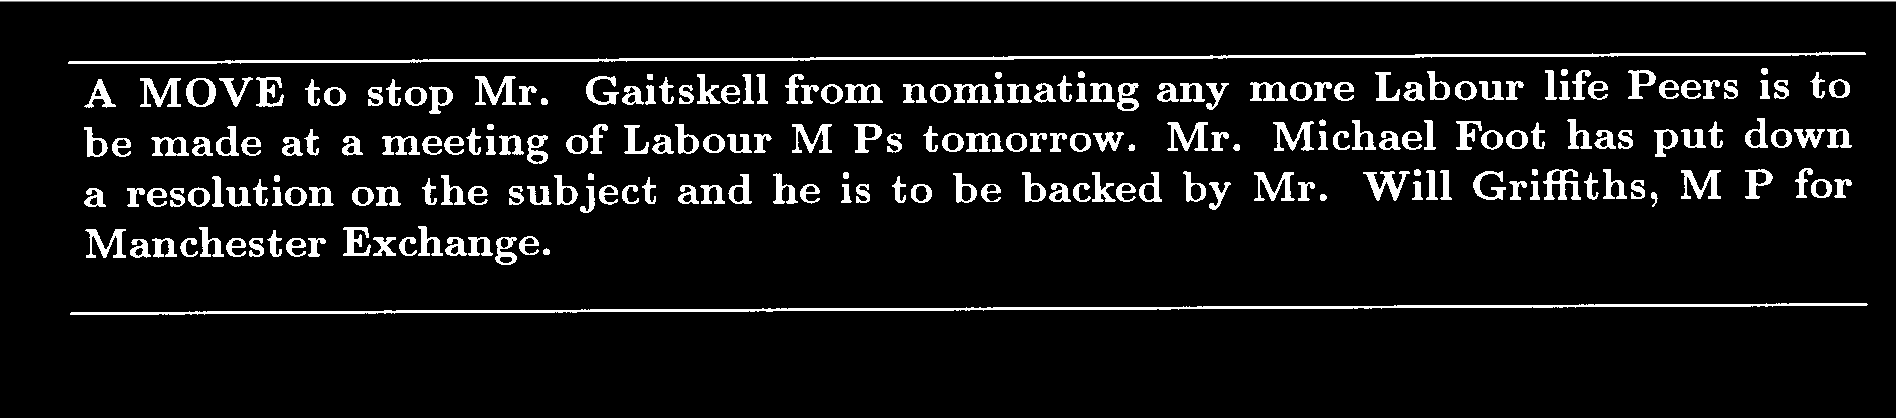
\includegraphics[width=\textwidth]{PreprocessedImg.PNG}
		\caption{preprocessed image}
		\label{fig:ex2a}
	\end{subfigure}
	\begin{subfigure}{0.40\textwidth}
		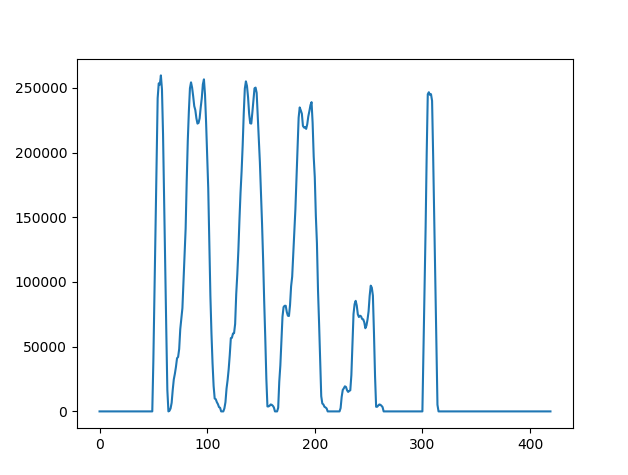
\includegraphics[width=\textwidth]{HorzProjection.PNG}
		\caption{horizontal projection profile}
		\label{fig:ex2b}
	\end{subfigure}
	\caption{Example of a preprocessed image and line projection profile.}
	\label{fig:ex_proj_horz}
\end{figure}

\begin{figure}
	\centering
	\begin{subfigure}{0.40\textwidth}
		
\includegraphics[width=\textwidth]{PreprocessedLine.PNG}
		\caption{preprocessed image}
		\label{fig:ex2a}
	\end{subfigure}
	\begin{subfigure}{0.40\textwidth}
		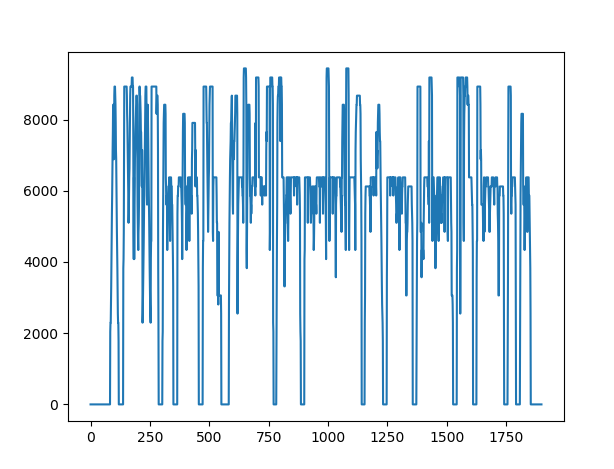
\includegraphics[width=\textwidth]{VertProjectionWord.PNG}
		\caption{horizontal projection profile}
		\label{fig:ex2b}
	\end{subfigure}
	\caption{Example of a further dilated extracted line and word projection profile.}
	\label{fig:ex_proj_vert}
\end{figure}

In the last step, the detected words are segmented into characters. Some characters have a distance of one pixel on the closest point. Therefore, an Otsu-threshold is applied and inverted, without any dilation and blurring. 
An example of is shown in Figure \ref{fig:ex_proj_vert_char}.
The line and word segmentation work flawless, but the character segmentation has some failures.
We first tried to use the preprocessed image, which we used for the other segmentation.
Though, this leads to merged characters in many cases, as visible in Figure \ref{fig:ex_merged_characters}.
We tried the same without dilation, but that yields the same results, because of the blur which already merges the characters.

\begin{figure}
	\centering
	\begin{subfigure}{0.40\textwidth}
		
\includegraphics[width=\textwidth]{PreprocessedWord.PNG}
		\caption{preprocessed image}
		\label{fig:ex2a}
	\end{subfigure}
	\begin{subfigure}{0.40\textwidth}
		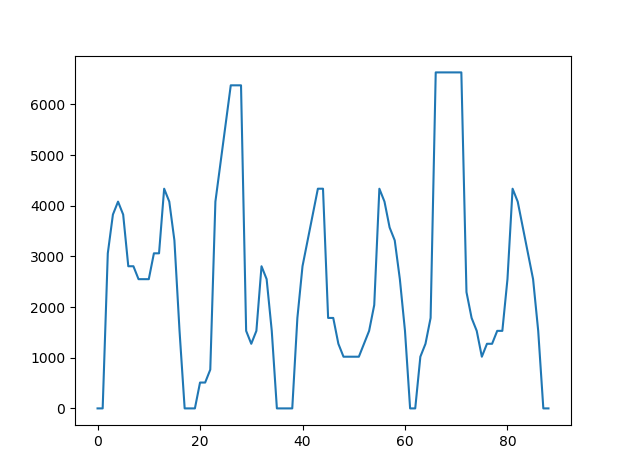
\includegraphics[width=\textwidth]{VertProjectionChar.PNG}
		\caption{horizontal projection profile}
		\label{fig:ex2b}
	\end{subfigure}
	\caption{Example images of an extracted word without blurring and dilating and its vertical projection profile.}
	\label{fig:ex_proj_vert_char}
\end{figure}

\begin{figure}
	\centering
	\begin{subfigure}{0.2\textwidth}
		
\includegraphics[width=\textwidth]{mergedChars1.PNG}
		\label{fig:ex2a}
	\end{subfigure}
	\begin{subfigure}{0.30\textwidth}
		
\includegraphics[width=\textwidth]{mergedChars2.PNG}
		\label{fig:ex2b}
	\end{subfigure}
	\begin{subfigure}{0.25\textwidth}
		
\includegraphics[width=\textwidth]{mergedChars3.PNG}
		\label{fig:ex2b}
	\end{subfigure}
	\caption{Example images of merged characters.}
	\label{fig:ex_merged_characters}
\end{figure}

Another approach uses skeletonization.
This method works quite good to resolve the merged characters. Though, it has the disadvantage of split characters because of thin characters, as visible in Figure \ref{fig:ex_split_characters}.
For this reason, we rejected this approach as it introduces more errors. 
Our final method uses no blur and no dilation and works on the original image, with an applied threshold and inverted.
The top and bottom space are cut to remove overlaps from other characters, for example, the character 'f', and the 
vertical projection profile is applied afterward. With this approach, we achieve the correct results in about 90 \% of the cases.
Some errors remain, especially if characters are connected or overlap.

\begin{figure}
	\centering
	\begin{subfigure}{0.05\textwidth}
		
\includegraphics[width=\textwidth]{splitChars1.PNG}
		\label{fig:ex2a}
	\end{subfigure}
	\begin{subfigure}{0.05\textwidth}
		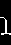
\includegraphics[width=\textwidth]{splitChars2.PNG}
		\label{fig:ex2b}
	\end{subfigure}
	\begin{subfigure}{0.1\textwidth}
		
\includegraphics[width=\textwidth]{splitChars3.PNG}
		\label{fig:ex2b}
	\end{subfigure}
	\caption{Example images of split characters.}
	\label{fig:ex_split_characters}
\end{figure}

\subsection{Convolutional Neural Network}

The prediction of the letters is done using a trained convolutional neural network. The network configuration and parameters are trained using generated training data. This data consists of randomly generated letters and digits in randomly chosen fonts.

Each image of the training data has 28 x 28 pixels for the network as input. The generated and detected letters are cropped, padded to square images (to preserve the aspect ratio) and scaled. This leads to scale-invariant character recognition. For convenience, the letters are saved as images and a TSV-file labels the images with the corresponding letter and letter-index.

The neural network consists of multiple convolution, pooling, and dropout-layers. In the end the classification is achieved using a flattened and dense network with a soft-max-function to result in probabilities. The exact structure of the network is shown in the following code listing.

\begin{lstlisting}
_________________________________________________________________
Layer (type)                 Output Shape              Param #   
=================================================================
conv2d_1 (Conv2D)            (None, 26, 26, 32)        320       
_________________________________________________________________
conv2d_2 (Conv2D)            (None, 24, 24, 64)        18496     
_________________________________________________________________
max_pooling2d_1 (MaxPooling2 (None, 12, 12, 64)        0         
_________________________________________________________________
dropout_1 (Dropout)          (None, 12, 12, 64)        0         
_________________________________________________________________
flatten_1 (Flatten)          (None, 9216)              0         
_________________________________________________________________
dense_1 (Dense)              (None, 128)               1179776   
_________________________________________________________________
dropout_2 (Dropout)          (None, 128)               0         
_________________________________________________________________
dense_2 (Dense)              (None, 64)                8256      
=================================================================
Total params: 1,206,848
Trainable params: 1,206,848
Non-trainable params: 0
_________________________________________________________________
\end{lstlisting}

Currently, the maximum of the probabilities of possible letters is taken to determine the letter. A future approach could use this probability for a dictionary to correct minor mistakes.

\section{Evaluation and Results}

To measure the performance the Levenshtein distance measure is used to compare the predicted text with the ground truth. Since the text length varies in the dataset, this distance is divided by the text-length to compare them and average them. Overall, an average of 0.11 edits per letter is achieved. This means that a predicted text of 100 letters needs 11 edits to be equal to the ground truth. This error includes the errors from the letter prediction, but also the error of the segmentation since wrong segmented parts are misclassified as well. This is especially a problem for connected letters.

A detailed view of the misclassified letters, reveals that the letters 'O' and the punctuation mark '.' is confused, since both get cropped and scaled to the same resolution. Future implementations should focus on preserving the relative size of the letter in contrast to the line as well. 

Punctuation marks are a problem in general since the current version is only trained for dots and commas. This leads to a confusion of double quotation marks with two regular ones, for example. Punctuation marks should either be detected separately or preserved in size, as stated above.

\bibliographystyle{plain}
\bibliography{lit}
%% References can be stored in a seperate bib-file (see lit.bib). References, that are cited in the report using \cite are automatically added to the reference list. For more information: http://www.bibtex.org/Using/
%%------------------------------------------------------
\end{document}
